% Standalone print cover for an A5 softcover with an 11 mm spine.
% Final size with bleed: 313 mm x 216 mm.
% Compile from the repository root with: latexmk cover.tex
\documentclass{article}

\usepackage[
    paperwidth=313mm,
    paperheight=216mm,
    margin=0mm,
    noheadfoot
]{geometry}
\usepackage{fontspec}
\usepackage{lmodern}
\usepackage{graphicx}
\usepackage{tikz}
\usepackage{xcolor}
\usepackage{microtype}
\usepackage[normalem]{ulem}

\definecolor{seeblau100}{RGB}{0,169,224}
\newcommand{\seeblauuline}[1]{{\renewcommand{\ULthickness}{1.2pt}\textcolor{seeblau100}{\uline{\textcolor{black}{#1}}}}}
\pagestyle{empty}
\setlength{\parindent}{0pt}

% Print geometry. The trim is 3 mm inside the PDF edge.
\newcommand{\Bleed}{3mm}
\newcommand{\PanelWidth}{148mm}
\newcommand{\SpineWidth}{11mm}

% Set this to \showcoverguidestrue for a proof PDF with construction guides.
\newif\ifshowcoverguides
\showcoverguidesfalse

\begin{document}
\begin{tikzpicture}[remember picture,overlay,x=1mm,y=1mm]
\begin{scope}[shift={(current page.south west)}]
    % Continuous artwork extends across the complete bleed area.
    \node[anchor=center,inner sep=0pt] at (156.5,108) {%
        \includegraphics[height=216mm]{utilities/configuration_ultra.jpg}%
    };

    % Reproduce the left-aligned crop used by the online back cover.
    \begin{scope}
        \clip (0,0) rectangle (151,216);
        \node[anchor=west,inner sep=0pt] at (0,108) {%
            \includegraphics[height=216mm]{utilities/configuration_ultra.jpg}%
        };
    \end{scope}

    % Front cover, right panel.
    \node[anchor=north east,inner sep=0pt] at (305,207) {%
        
\includegraphics[width=55mm]{utilities/uni logo/UniKonstanz_Logo_Optimum.pdf}%
    };

    \node[
        anchor=center,
        align=center,
        text width=122mm,
        font=\sffamily\bfseries\fontsize{16}{19}\selectfont
    ] at (236,151) {%
        \seeblauuline{Microwave Driven Transport in}\\
        \seeblauuline{Mesoscopic Superconducting Junctions}\\
        \seeblauuline{from Tunnel Barriers to Atomic Contacts}
    };

    \node[
        anchor=south,
        align=center,
        text width=120mm,
        font=\sffamily\bfseries\fontsize{16}{19}\selectfont
    ] at (236,18) {Oliver Aschenbrenner};

    % Spine. The pale strip improves contrast without hiding the artwork.
    \fill[white,opacity=0.70] (152,0) rectangle (161,216);
    \node[
        rotate=90,
        anchor=center,
        align=center,
        text width=184mm,
        font=\sffamily\bfseries\fontsize{10}{12}\selectfont
    ] at (156.5,108) {Oliver Aschenbrenner\quad\textbullet\quad Microwave Driven Transport in Mesoscopic Superconducting Junctions};

    % Back cover, left panel.
    \fill[white,opacity=0.88] (8,84) rectangle (146,132);
    \node[anchor=north west,inner sep=0pt] at (13,127) {%
        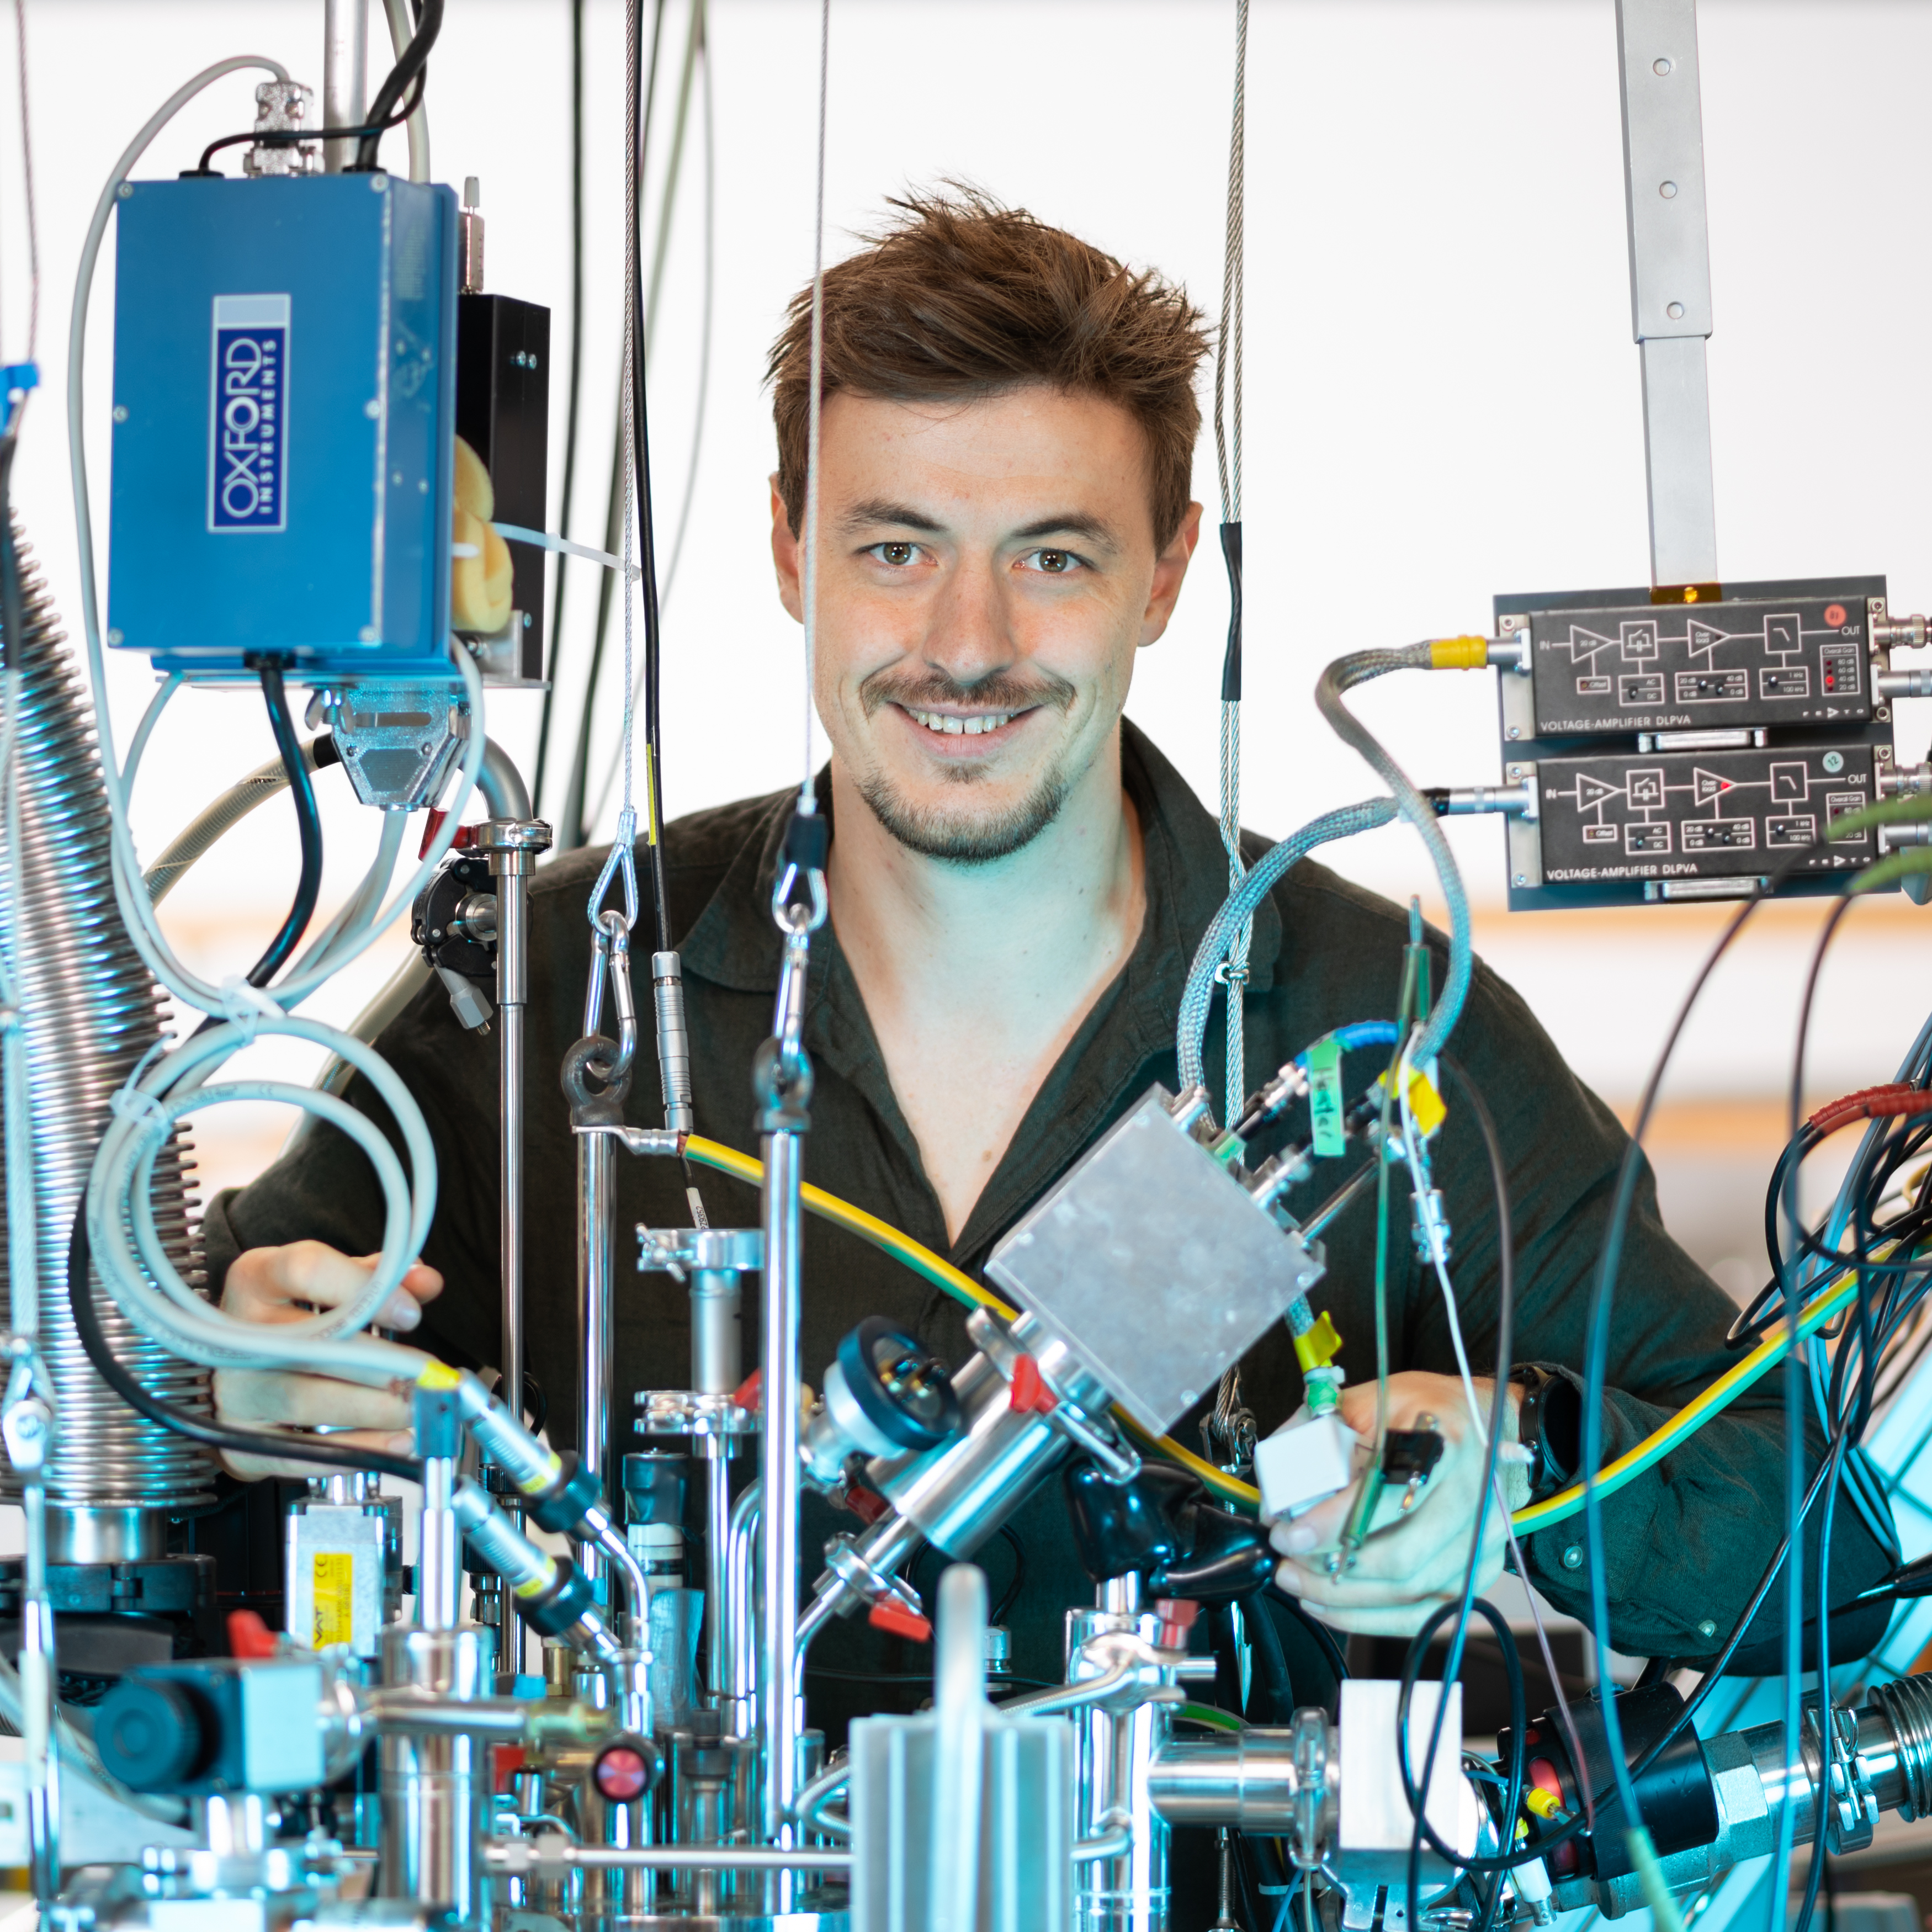
\includegraphics[width=38mm]{miscellaneous/backcover/portrait.jpg}%
    };
    \node[
        anchor=north west,
        inner sep=0pt
    ] at (56,127) {%
        \begin{minipage}{85mm}
            \sffamily\fontsize{9}{12.42}\selectfont
            \looseness=-1
            Oliver Aschenbrenner studies quantum transport in mesoscopic superconducting devices. In the group of Prof.~Dr.~Elke Scheer at the University of Konstanz, he investigates microwave driven transport from tunnel junctions to atomic contacts. His work combines low-temperature experiments, nanofabrication, automated measurements, and quantitative transport models. He earned his bachelor's and master's degrees in physics at the University of Konstanz and gained research experience at Ume\aa{} University and the University of Zagreb.
        \end{minipage}%
    };

    % Optional nonprinting proof guides.
    \ifshowcoverguides
        % Trim boundary.
        \draw[magenta,line width=0.35mm,dashed] (3,3) rectangle (310,213);
        % Spine folds after the 148 mm back panel and before the front panel.
        \draw[magenta,line width=0.25mm] (151,3) -- (151,213);
        \draw[magenta,line width=0.25mm] (162,3) -- (162,213);
        % Five millimeter safety areas inside the back and front trim.
        \draw[cyan,line width=0.25mm,dashed] (8,8) rectangle (146,208);
        \draw[cyan,line width=0.25mm,dashed] (167,8) rectangle (305,208);
        \node[anchor=south west,fill=white,font=\sffamily\scriptsize] at (4,4) {Proof guides only. Disable before print export.};
    \fi
\end{scope}
\end{tikzpicture}
\null
\newpage

% Inner cover spread. U2 is on the left and U3 is on the right.
\begin{tikzpicture}[remember picture,overlay,x=1mm,y=1mm]
\begin{scope}[shift={(current page.south west)}]
    % U2 reproduces the publication-information page from the online version.
    \node[
        anchor=north west,
        inner sep=0pt
    ] at (23,193) {%
        \begin{minipage}{120mm}
            \sffamily\fontsize{9}{12.42}\selectfont
            Dissertation der Universit\"at Konstanz\\[12.42pt]
            Tag der m\"undlichen Pr\"ufung: 8. Oktober 2026\\[12.42pt]
            1. Referentin: Prof. Dr. Elke Scheer\\
            2. Referent: Prof. Dr. Angelo Di Bernardo
        \end{minipage}%
    };

    \node[
        anchor=north west,
        inner sep=0pt,
        font=\sffamily\bfseries\fontsize{9}{12.42}\selectfont
    ] at (23,33) {Cover:};

    \node[
        anchor=north west,
        inner sep=0pt
    ] at (38,33) {%
        \begin{minipage}{85mm}
            \sffamily\fontsize{9}{12.42}\selectfont
            Rendering of an atomic contact.\\
            Calculations performed by\\
            Markus Ring and David Weber.
        \end{minipage}%
    };

    % U3 intentionally remains empty.
    \ifshowcoverguides
        \draw[magenta,line width=0.35mm,dashed] (3,3) rectangle (310,213);
        \draw[magenta,line width=0.25mm] (151,3) -- (151,213);
        \draw[magenta,line width=0.25mm] (162,3) -- (162,213);
        \draw[cyan,line width=0.25mm,dashed] (8,8) rectangle (146,208);
        \draw[cyan,line width=0.25mm,dashed] (167,8) rectangle (305,208);
        \node[anchor=south west,fill=white,font=\sffamily\scriptsize] at (4,4) {Proof guides only. Disable before print export.};
    \fi
\end{scope}
\end{tikzpicture}
\null
\end{document}
